\chapter{Witness Domain Implementation}
\label{ch:witness-domain-implementation}

\section{Why battery is the witness domain}
Battery remains the witness domain because it is the clearest place in the repository where
the full ORIUS stack can be seen at once: degraded telemetry, reliability estimation,
uncertainty inflation, repaired dispatch, fallback behavior, certificate traces, replayable
fault schedules, and claim-locked artifact surfaces. That makes it the right row to
demonstrate end-to-end doctrine closure without allowing the dissertation to collapse into
an energy-only story.

The witness role is methodological rather than rhetorical. Battery is not the identity of
ORIUS. It is the row in which the theorem layer, the implementation layer, and the artifact
layer are all strong enough to support the book's deepest defended argument.

\section{Witness-domain problem and plant semantics}
The battery plant exposes a particularly clear form of OASG. Dispatch legality is computed
against observed state of charge, availability, and feeder conditions, but the physical
asset evolves on the true state. When telemetry becomes stale or corrupted, the optimizer
can continue to return actions that appear feasible on the observed state while the physical
asset is already drifting toward an unsafe or infeasible region.

That clarity is useful for a witness row because it makes visible what ORIUS actually
changes: the release boundary, not merely the forecast. The runtime widens the
observation-consistent state, recomputes admissible dispatch, repairs or curtails candidate
action, and emits a certificate describing why release remains justified.

\section{Data surfaces and dataset cards}
The witness row is artifact-first rather than repository-inline. The battery surface is
therefore described through tracked dataset cards, manifests, and publication artifacts
instead of through the fiction that all raw data live inside the git tree. That design is
not a weakness. It is how a dissertation remains reproducible when its empirical surface
depends on large external or governed datasets.

\IfFileExists{paper/assets/tables/generated/tbl07_dataset_cards.tex}{%
\begin{table*}[htbp]
\centering
\small
\caption{Dataset-card inventory for the four evaluation regions.}
\label{tab:TBL07_DATASET_CARDS}
\setlength{\tabcolsep}{4pt}
\renewcommand{\arraystretch}{1.10}
\resizebox{\linewidth}{!}{%
\begin{tabular}{llrrlrll}
\toprule
\textbf{Dataset} & \textbf{Country} & \textbf{Rows} & \textbf{Features} & \textbf{Period} & \textbf{Coverage (\%)} & \textbf{Source} & \textbf{Carbon Source} \\
\midrule
Germany (OPSD) & DE & 17,377 & 94 & 2018-10-07 -- 2020-09-30 & 100.0 & OPSD + SMARD & SMARD generation mix \\
USA (EIA-930 ERCOT) & US & 13,453 & 62 & 2024-07-01 -- 2026-01-20 & 100.0 & EIA-930 ERCOT & proxy\_generation\_mix \\
USA (EIA-930 MISO) & US & 13,638 & 114 & 2024-07-01 -- 2026-01-20 & 100.0 & EIA-930 MISO & proxy\_generation\_mix \\
USA (EIA-930 PJM) & US & 13,639 & 62 & 2024-07-01 -- 2026-01-20 & 100.0 & EIA-930 PJM & proxy\_generation\_mix \\
\bottomrule
\end{tabular}
}
\end{table*}%
}{%
\begin{table*}[htbp]
\centering
\small
\caption{Dataset-card inventory for the four evaluation regions.}
\label{tab:TBL07_DATASET_CARDS}
\setlength{\tabcolsep}{4pt}
\renewcommand{\arraystretch}{1.10}
\resizebox{\linewidth}{!}{%
\begin{tabular}{llrrlrll}
\toprule
\textbf{Dataset} & \textbf{Country} & \textbf{Rows} & \textbf{Features} & \textbf{Period} & \textbf{Coverage (\%)} & \textbf{Source} & \textbf{Carbon Source} \\
\midrule
Germany (OPSD) & DE & 17,377 & 94 & 2018-10-07 -- 2020-09-30 & 100.0 & OPSD + SMARD & SMARD generation mix \\
USA (EIA-930 ERCOT) & US & 13,453 & 62 & 2024-07-01 -- 2026-01-20 & 100.0 & EIA-930 ERCOT & proxy\_generation\_mix \\
USA (EIA-930 MISO) & US & 13,638 & 114 & 2024-07-01 -- 2026-01-20 & 100.0 & EIA-930 MISO & proxy\_generation\_mix \\
USA (EIA-930 PJM) & US & 13,639 & 62 & 2024-07-01 -- 2026-01-20 & 100.0 & EIA-930 PJM & proxy\_generation\_mix \\
\bottomrule
\end{tabular}
}
\end{table*}%
}

The dataset-card layer does more than document provenance. It tells the reader which
geographies, telemetry resolutions, market structures, and operating contexts actually
support the witness claim. That keeps the battery row from drifting into a false claim of
energy-system universality.

\section{Forecasting, calibration, and reliability surfaces}
The witness row deliberately separates three roles that are often blurred in energy papers:
\begin{enumerate}
  \item the forecasting surface that supports nominal dispatch;
  \item the uncertainty or calibration surface that informs admissible release; and
  \item the reliability surface that decides how aggressively the runtime must tighten
  action when telemetry degrades.
\end{enumerate}

That separation matters because ORIUS is not strongest where it finds the best forecaster.
It is strongest where reliability, uncertainty, repair, and certificate semantics can be
shown working together on one defended row.

\IfFileExists{paper/assets/tables/generated/tbl08_forecast_baselines.tex}{%
\begin{table}[htbp]
\centering
\small
\caption{Six-model forecast comparison (DE \& US). GBM dominates across all targets. PICP/Width shown only for GBM (production conformal intervals). Negative $R^2$ indicates worse-than-mean predictions.}
\label{tab:TBL08_FORECAST_BASELINES}
\setlength{\tabcolsep}{3pt}
\renewcommand{\arraystretch}{0.98}
\resizebox{\linewidth}{!}{%
\begin{tabular}{lllrrrrrr}
\toprule
\textbf{Region} & \textbf{Target} & \textbf{Model} & \textbf{RMSE} & \textbf{MAE} & \textbf{sMAPE (\%)} & $\mathbf{R^2}$ & \textbf{PICP@90} & \textbf{Width (MW)} \\
\midrule
DE & Load & \textbf{GBM} & \textbf{305.1} & \textbf{187.9} & \textbf{0.39} & \textbf{0.9988} & 88.2 & 1070.2 \\
DE & Load & LSTM & 1204.5 & 945.2 & 5.29 & 0.8408 & not appl. & not appl. \\
DE & Load & TCN & 902.0 & 713.6 & 4.25 & 0.9021 & not appl. & not appl. \\
DE & Load & N-BEATS & 715.8 & 558.9 & 3.61 & 0.9317 & not appl. & not appl. \\
DE & Load & TFT & 552.9 & 430.7 & 2.45 & 0.9433 & not appl. & not appl. \\
DE & Load & PatchTST & 491.4 & 387.6 & 2.26 & 0.9530 & not appl. & not appl. \\
\midrule
DE & Wind & \textbf{GBM} & \textbf{219.1} & \textbf{129.4} & \textbf{2.41} & \textbf{0.9991} & 93.7 & 833.9 \\
DE & Wind & LSTM & 850.5 & 662.0 & 83.69 & 0.8466 & not appl. & not appl. \\
DE & Wind & TCN & 737.7 & 585.0 & 103.77 & 0.8802 & not appl. & not appl. \\
DE & Wind & N-BEATS & 492.8 & 385.0 & 69.37 & 0.9368 & not appl. & not appl. \\
DE & Wind & TFT & 478.3 & 374.7 & 57.00 & 0.9450 & not appl. & not appl. \\
DE & Wind & PatchTST & 359.1 & 282.1 & 48.03 & 0.9627 & not appl. & not appl. \\
\midrule
DE & Solar & \textbf{GBM} & \textbf{240.3} & \textbf{117.3} & \textbf{69.24} & \textbf{0.9993} & 78.8 & 1037.7 \\
DE & Solar & LSTM & 977.0 & 770.9 & 235.10 & 0.8619 & not appl. & not appl. \\
DE & Solar & TCN & 836.7 & 655.4 & 175.57 & 0.8914 & not appl. & not appl. \\
DE & Solar & N-BEATS & 556.3 & 437.4 & 95.70 & 0.9424 & not appl. & not appl. \\
DE & Solar & TFT & 488.1 & 381.5 & 94.71 & 0.9506 & not appl. & not appl. \\
DE & Solar & PatchTST & 406.5 & 320.6 & 103.65 & 0.9543 & not appl. & not appl. \\
\midrule
US & Load & \textbf{GBM} & \textbf{183.4} & \textbf{140.6} & \textbf{0.18} & \textbf{0.9993} & 82.6 & 1986.8 \\
US & Load & LSTM & 671.7 & 529.9 & 3.42 & 0.8430 & not appl. & not appl. \\
US & Load & TCN & 595.0 & 463.6 & 2.60 & 0.8909 & not appl. & not appl. \\
US & Load & N-BEATS & 367.6 & 292.4 & 1.68 & 0.9353 & not appl. & not appl. \\
US & Load & TFT & 377.6 & 295.8 & 1.93 & 0.9491 & not appl. & not appl. \\
US & Load & PatchTST & 346.9 & 274.1 & 1.68 & 0.9525 & not appl. & not appl. \\
\midrule
US & Wind & \textbf{GBM} & \textbf{357.1} & \textbf{210.7} & \textbf{2.65} & \textbf{0.9972} & 40.6 & 324.9 \\
US & Wind & LSTM & 1497.2 & 1168.1 & 180.11 & 0.8592 & not appl. & not appl. \\
US & Wind & TCN & 1171.0 & 911.8 & 117.98 & 0.9053 & not appl. & not appl. \\
US & Wind & N-BEATS & 719.4 & 563.0 & 80.58 & 0.9306 & not appl. & not appl. \\
US & Wind & TFT & 681.0 & 533.6 & 81.35 & 0.9432 & not appl. & not appl. \\
US & Wind & PatchTST & 696.5 & 548.8 & 98.79 & 0.9547 & not appl. & not appl. \\
\midrule
US & Solar & \textbf{GBM} & \textbf{230.0} & \textbf{82.1} & \textbf{53.09} & \textbf{0.9947} & 86.5 & 687.0 \\
US & Solar & LSTM & 868.7 & 691.0 & 151.85 & 0.8674 & not appl. & not appl. \\
US & Solar & TCN & 686.6 & 545.8 & 113.95 & 0.8874 & not appl. & not appl. \\
US & Solar & N-BEATS & 467.2 & 368.5 & 76.08 & 0.9417 & not appl. & not appl. \\
US & Solar & TFT & 450.7 & 351.4 & 103.59 & 0.9433 & not appl. & not appl. \\
US & Solar & PatchTST & 414.9 & 323.1 & 88.50 & 0.9514 & not appl. & not appl. \\
\bottomrule
\end{tabular}
}
\end{table}%
}{%
\begin{table}[htbp]
\centering
\small
\caption{Six-model forecast comparison (DE \& US). GBM dominates across all targets. PICP/Width shown only for GBM (production conformal intervals). Negative $R^2$ indicates worse-than-mean predictions.}
\label{tab:TBL08_FORECAST_BASELINES}
\setlength{\tabcolsep}{3pt}
\renewcommand{\arraystretch}{0.98}
\resizebox{\linewidth}{!}{%
\begin{tabular}{lllrrrrrr}
\toprule
\textbf{Region} & \textbf{Target} & \textbf{Model} & \textbf{RMSE} & \textbf{MAE} & \textbf{sMAPE (\%)} & $\mathbf{R^2}$ & \textbf{PICP@90} & \textbf{Width (MW)} \\
\midrule
DE & Load & \textbf{GBM} & \textbf{305.1} & \textbf{187.9} & \textbf{0.39} & \textbf{0.9988} & 88.2 & 1070.2 \\
DE & Load & LSTM & 1204.5 & 945.2 & 5.29 & 0.8408 & not appl. & not appl. \\
DE & Load & TCN & 902.0 & 713.6 & 4.25 & 0.9021 & not appl. & not appl. \\
DE & Load & N-BEATS & 715.8 & 558.9 & 3.61 & 0.9317 & not appl. & not appl. \\
DE & Load & TFT & 552.9 & 430.7 & 2.45 & 0.9433 & not appl. & not appl. \\
DE & Load & PatchTST & 491.4 & 387.6 & 2.26 & 0.9530 & not appl. & not appl. \\
\midrule
DE & Wind & \textbf{GBM} & \textbf{219.1} & \textbf{129.4} & \textbf{2.41} & \textbf{0.9991} & 93.7 & 833.9 \\
DE & Wind & LSTM & 850.5 & 662.0 & 83.69 & 0.8466 & not appl. & not appl. \\
DE & Wind & TCN & 737.7 & 585.0 & 103.77 & 0.8802 & not appl. & not appl. \\
DE & Wind & N-BEATS & 492.8 & 385.0 & 69.37 & 0.9368 & not appl. & not appl. \\
DE & Wind & TFT & 478.3 & 374.7 & 57.00 & 0.9450 & not appl. & not appl. \\
DE & Wind & PatchTST & 359.1 & 282.1 & 48.03 & 0.9627 & not appl. & not appl. \\
\midrule
DE & Solar & \textbf{GBM} & \textbf{240.3} & \textbf{117.3} & \textbf{69.24} & \textbf{0.9993} & 78.8 & 1037.7 \\
DE & Solar & LSTM & 977.0 & 770.9 & 235.10 & 0.8619 & not appl. & not appl. \\
DE & Solar & TCN & 836.7 & 655.4 & 175.57 & 0.8914 & not appl. & not appl. \\
DE & Solar & N-BEATS & 556.3 & 437.4 & 95.70 & 0.9424 & not appl. & not appl. \\
DE & Solar & TFT & 488.1 & 381.5 & 94.71 & 0.9506 & not appl. & not appl. \\
DE & Solar & PatchTST & 406.5 & 320.6 & 103.65 & 0.9543 & not appl. & not appl. \\
\midrule
US & Load & \textbf{GBM} & \textbf{183.4} & \textbf{140.6} & \textbf{0.18} & \textbf{0.9993} & 82.6 & 1986.8 \\
US & Load & LSTM & 671.7 & 529.9 & 3.42 & 0.8430 & not appl. & not appl. \\
US & Load & TCN & 595.0 & 463.6 & 2.60 & 0.8909 & not appl. & not appl. \\
US & Load & N-BEATS & 367.6 & 292.4 & 1.68 & 0.9353 & not appl. & not appl. \\
US & Load & TFT & 377.6 & 295.8 & 1.93 & 0.9491 & not appl. & not appl. \\
US & Load & PatchTST & 346.9 & 274.1 & 1.68 & 0.9525 & not appl. & not appl. \\
\midrule
US & Wind & \textbf{GBM} & \textbf{357.1} & \textbf{210.7} & \textbf{2.65} & \textbf{0.9972} & 40.6 & 324.9 \\
US & Wind & LSTM & 1497.2 & 1168.1 & 180.11 & 0.8592 & not appl. & not appl. \\
US & Wind & TCN & 1171.0 & 911.8 & 117.98 & 0.9053 & not appl. & not appl. \\
US & Wind & N-BEATS & 719.4 & 563.0 & 80.58 & 0.9306 & not appl. & not appl. \\
US & Wind & TFT & 681.0 & 533.6 & 81.35 & 0.9432 & not appl. & not appl. \\
US & Wind & PatchTST & 696.5 & 548.8 & 98.79 & 0.9547 & not appl. & not appl. \\
\midrule
US & Solar & \textbf{GBM} & \textbf{230.0} & \textbf{82.1} & \textbf{53.09} & \textbf{0.9947} & 86.5 & 687.0 \\
US & Solar & LSTM & 868.7 & 691.0 & 151.85 & 0.8674 & not appl. & not appl. \\
US & Solar & TCN & 686.6 & 545.8 & 113.95 & 0.8874 & not appl. & not appl. \\
US & Solar & N-BEATS & 467.2 & 368.5 & 76.08 & 0.9417 & not appl. & not appl. \\
US & Solar & TFT & 450.7 & 351.4 & 103.59 & 0.9433 & not appl. & not appl. \\
US & Solar & PatchTST & 414.9 & 323.1 & 88.50 & 0.9514 & not appl. & not appl. \\
\bottomrule
\end{tabular}
}
\end{table}%
}

\IfFileExists{paper/assets/tables/generated/tbl_battery_deep_oqe_summary.tex}{%
\begin{table}[ht]
\centering
\caption{Battery DeepOQE diagnostics on the held-out degraded-telemetry episodes.}
\label{tab:battery-deep-oqe-summary}
\begin{tabular}{lrr}
\toprule
Metric & Heuristic & DeepOQE \\
\midrule
Reliability MAE & 0.1176 & 0.1613 \\
Fault AUC & not appl. & 0.5383 \\
Low-reliability fault lift & not appl. & 136.821 \\
\bottomrule
\end{tabular}
\end{table}
%
}{%
\begin{table}[ht]
\centering
\caption{Battery DeepOQE diagnostics on the held-out degraded-telemetry episodes.}
\label{tab:battery-deep-oqe-summary}
\begin{tabular}{lrr}
\toprule
Metric & Heuristic & DeepOQE \\
\midrule
Reliability MAE & 0.1176 & 0.1613 \\
Fault AUC & not appl. & 0.5383 \\
Low-reliability fault lift & not appl. & 136.821 \\
\bottomrule
\end{tabular}
\end{table}
%
}

\begin{figure}[htbp]
\centering
\IfFileExists{reports/publication/fig_battery_reliability_baselines.png}{%
\includegraphics[width=0.84\textwidth]{reports/publication/fig_battery_reliability_baselines.png}%
}{%
\includegraphics[width=0.84\textwidth]{../reports/publication/fig_battery_reliability_baselines.png}%
}
\caption{Witness-domain reliability baselines. The engineered forecasting surface and the
learned reliability surface are intentionally reported together so the dissertation does not
confuse forecasting novelty with degraded-observation novelty.}
\label{fig:witness-reliability-baselines}
\end{figure}

Taken together, the tables and figure support a bounded but important point. Even when deep
forecasting does not dominate the engineered tabular baseline, learned reliability remains a
scientifically relevant extension because ORIUS cares about release under degraded sensing,
not only about point prediction quality.

\section{Control baselines and adapter implementation}
Battery is also the cleanest row for showing the adapter boundary in operational terms. The
adapter binds:
\begin{itemize}
  \item telemetry parsing and state semantics;
  \item the true-state safety predicate;
  \item dispatch feasibility and repair geometry;
  \item certificate payload fields; and
  \item the bounded fallback policy used when admissible repaired action disappears.
\end{itemize}
This is where the implementation philosophy becomes concrete. The nominal forecasting and
optimization stack can vary, but the ORIUS adapter contract and replay schema remain fixed.

\section{Locked artifact protocol}
The witness row is defended through locked artifacts rather than narrative memory. Training
surfaces, replay outputs, theorem traces, calibration diagnostics, deep-reliability
summaries, runtime tables, and parity surfaces all point back to generated publication
artifacts or manifests. This is where the chapter-first dissertation model and the
repository's claim-lock machinery meet: the prose is curated, but the evidence remains
machine-governed.

\section{Witness-row scope}
Battery carries the book's deepest defended claim because it closes the full runtime-safety
chain from degraded observation to governed release. It does not prove that every battery
chemistry, market policy, or asset-health objective is universally solved. Instead, it gives
the dissertation a calibration surface: one row where theorem, runtime, and artifact closure
can all be inspected together before the argument is lifted across domains.
